% Documents setup
\documentclass[11pt]{book}

% fix for pandoc 1.14
\providecommand{\tightlist}{%
  \setlength{\itemsep}{0pt}\setlength{\parskip}{0pt}}

\usepackage{tabu} % https://tex.stackexchange.com/questions/50332/vertical-spacing-of-a-table-cell

% Location of the csas-style repository: adjust path as needed
\newcommand{\locRepo}{csas-style}

% Use the style file in the csas-style repository (res-doc.sty)
\usepackage{\locRepo/res-doc}

% header-includes from R markdown entry


% Headers and footers
\lhead{Draft working paper --- Do not cite or circulate}
% \lhead{}
\rhead{}
% \rfoot{DRAFT - DO NOT CITE}

%%%% Commands for title page etc %%%%%

% Publication year
\newcommand{\rdYear}{2021}

% Publication month
\newcommand{\rdMonth}{Month}

% Report number
\newcommand{\rdNumber}{nnn}

% Region
\newcommand{\rdRegion}{Pacific Region}

% Title
\newcommand{\rdTitle}{Case Study Applications of LRP Estimation Methods to Pacific Salmon Stock Management Units}

\newcommand{\rdISBN}{}
\newcommand{\rdCatNo}{}

% Author names separated by commas and ', and' for the last author in the format 'M.H. Grinnell' (use \textsuperscript{n} for addresses)
\newcommand{\rdAuth}{First. M. Last\textsuperscript{1} and Alex B. Smith\textsuperscript{2}}

% Author names reversed separated by commas in the format 'Grinnell, M.H.'
\newcommand{\rdAuthRev}{Last, F.M. and Smith, A.B.}

% Author addresses (use \textsuperscript{n})
\newcommand{\rdAuthAddy}{\textsuperscript{1}Pacific Biological Station\\
Fisheries and Oceans Canada, 3190 Hammond Bay Road\\
Nanaimo, British Columbia, V9T 6N7, Canada\\
\textsuperscript{2}Far, far away\\
Another Galaxy}

\newcommand{\citationOtherLanguage}{Last, F.M. et Smith, A.B. Title Here (\emph{Latin Species Name}). DFO Secr. can. de consult. sci. du MPO. Doc. de rech 2019/nnn. iv + 13 p.}

% Name of file with abstract and resume (see \abstract and \frenchabstract for requirements)
\newcommand{\rdAbstract}{\abstract{Here is the abstract text. Lorem ipsum dolor sit amet, consectetur adipisicing elit, sed do eiusmod tempor incididunt ut labore et dolore magna aliqua. Ut enim ad minim veniam, quis nostrud exercitation ullamco laboris nisi ut aliquip ex ea commodo consequat. Duis aute irure dolor in reprehenderit in voluptate velit esse cillum dolore eu fugiat nulla pariatur. Excepteur sint occaecat cupidatat non proident, sunt in culpa qui officia deserunt mollit anim id est laborum. \vspace{1.5mm} \break Start new paragraphs after a blank line and with 2 spaces indent. Lorem ipsum dolor sit amet, consectetur adipisicing elit, sed do eiusmod tempor incididunt ut labore et dolore magna aliqua. Ut enim ad minim veniam, quis nostrud exercitation ullamco laboris nisi ut aliquip ex ea commodo consequat. Duis aute irure dolor in reprehenderit in voluptate velit esse cillum dolore eu fugiat nulla pariatur. Excepteur sint occaecat cupidatat non proident, sunt in culpa qui officia deserunt mollit anim id est laborum.}}

%%%% End of title page commands %%%%%

% \pdfcompresslevel=5 % faster PNGs

\setcounter{section}{0}

\bibliographystyle{csas-style/res-doc}

\usepackage{amsmath}
\usepackage{bm}

% commands and environments needed by pandoc snippets
% extracted from the output of `pandoc -s`
%% Make R markdown code chunks work
\usepackage{array}
\usepackage{amssymb,amsmath}
\usepackage{color}
\usepackage{fancyvrb}

% From default template:
\newcommand{\VerbBar}{|}
\newcommand{\VERB}{\Verb[commandchars=\\\{\}]}
\DefineVerbatimEnvironment{Highlighting}{Verbatim}{commandchars=\\\{\}}
% Add ',fontsize=\small' for more characters per line
\usepackage{framed}
\definecolor{shadecolor}{RGB}{248,248,248}
\newenvironment{Shaded}{\begin{snugshade}}{\end{snugshade}}
\newcommand{\AlertTok}[1]{\textcolor[rgb]{0.94,0.16,0.16}{#1}}
\newcommand{\AnnotationTok}[1]{\textcolor[rgb]{0.56,0.35,0.01}{\textbf{\textit{#1}}}}
\newcommand{\AttributeTok}[1]{\textcolor[rgb]{0.77,0.63,0.00}{#1}}
\newcommand{\BaseNTok}[1]{\textcolor[rgb]{0.00,0.00,0.81}{#1}}
\newcommand{\BuiltInTok}[1]{#1}
\newcommand{\CharTok}[1]{\textcolor[rgb]{0.31,0.60,0.02}{#1}}
\newcommand{\CommentTok}[1]{\textcolor[rgb]{0.56,0.35,0.01}{\textit{#1}}}
\newcommand{\CommentVarTok}[1]{\textcolor[rgb]{0.56,0.35,0.01}{\textbf{\textit{#1}}}}
\newcommand{\ConstantTok}[1]{\textcolor[rgb]{0.00,0.00,0.00}{#1}}
\newcommand{\ControlFlowTok}[1]{\textcolor[rgb]{0.13,0.29,0.53}{\textbf{#1}}}
\newcommand{\DataTypeTok}[1]{\textcolor[rgb]{0.13,0.29,0.53}{#1}}
\newcommand{\DecValTok}[1]{\textcolor[rgb]{0.00,0.00,0.81}{#1}}
\newcommand{\DocumentationTok}[1]{\textcolor[rgb]{0.56,0.35,0.01}{\textbf{\textit{#1}}}}
\newcommand{\ErrorTok}[1]{\textcolor[rgb]{0.64,0.00,0.00}{\textbf{#1}}}
\newcommand{\ExtensionTok}[1]{#1}
\newcommand{\FloatTok}[1]{\textcolor[rgb]{0.00,0.00,0.81}{#1}}
\newcommand{\FunctionTok}[1]{\textcolor[rgb]{0.00,0.00,0.00}{#1}}
\newcommand{\ImportTok}[1]{#1}
\newcommand{\InformationTok}[1]{\textcolor[rgb]{0.56,0.35,0.01}{\textbf{\textit{#1}}}}
\newcommand{\KeywordTok}[1]{\textcolor[rgb]{0.13,0.29,0.53}{\textbf{#1}}}
\newcommand{\NormalTok}[1]{#1}
\newcommand{\OperatorTok}[1]{\textcolor[rgb]{0.81,0.36,0.00}{\textbf{#1}}}
\newcommand{\OtherTok}[1]{\textcolor[rgb]{0.56,0.35,0.01}{#1}}
\newcommand{\PreprocessorTok}[1]{\textcolor[rgb]{0.56,0.35,0.01}{\textit{#1}}}
\newcommand{\RegionMarkerTok}[1]{#1}
\newcommand{\SpecialCharTok}[1]{\textcolor[rgb]{0.00,0.00,0.00}{#1}}
\newcommand{\SpecialStringTok}[1]{\textcolor[rgb]{0.31,0.60,0.02}{#1}}
\newcommand{\StringTok}[1]{\textcolor[rgb]{0.31,0.60,0.02}{#1}}
\newcommand{\VariableTok}[1]{\textcolor[rgb]{0.00,0.00,0.00}{#1}}
\newcommand{\VerbatimStringTok}[1]{\textcolor[rgb]{0.31,0.60,0.02}{#1}}
\newcommand{\WarningTok}[1]{\textcolor[rgb]{0.56,0.35,0.01}{\textbf{\textit{#1}}}}

\newcommand{\lt}{\ensuremath <}
\newcommand{\gt}{\ensuremath >}

%Defines cslreferences environment
%Required by pandoc 2.8
%Copied from https://github.com/rstudio/rmarkdown/issues/1649

\DeclareGraphicsExtensions{.png,.pdf}
\begin{document}

\frontmatter

\hypertarget{introduction}{%
\section{INTRODUCTION}\label{introduction}}
\begin{itemize}
\item
  This document supports the development of guidelines for defining LRPs for Pacific Salmon, as required by the recently revised Fisheries Act. Guidelines that have been informed by this work are available in the companion working paper ``Guidelines for Defining Limit Reference Points for Pacific Salmon Stock Management Units.''
\item
  Under the New Fisheries Act, Limit Reference Points (LRPs) that represent the level below which serious harm is occurring will be required for major fish stocks prescribed in regulation. For Pacific salmon, it is anticipated there could be \textgreater{} 65 major fish stocks (or stock management units, SMUs), where the proposed functional definition of a SMU is a group of one or more Wild Salmon Policy Conservation Units (CUs) that are managed together with the objective of achieving a joint status.
\item
  While lower biological benchmarks under the Wild Salmon Policy delineate abundances below which CUs are considered at risk of extinction (DFO 2005), these benchmarks have not been identified for many data-limited CUs and have not been aggregated to the SMU level, representing significant gaps in our ability to develop LRPs under the Fisheries Act.
\item
  The suite of LRP estimation methods considered in this paper are specific to the case where a LRP is defined as a single aggregate abundance that is associated with a high probability of all component CUs being above lower benchmarks that are consistent with the WSP. Alternative approaches to identifying LRPs are discussed in t
\item
  The overall goal of this working paper is demonstrate and evaluate LRPs for 3 case study stock management units. For each case study, the set of LRP estimation methods considered is a function of available data and previously developed assessment methods for the SMU.
\item
  In retrospective analyses, our objective is to demonstrate the sensitivity of the LRP to the removal of years or CUs to inform guidance about minimum numbers of years or CUs
\item
  In simulation evaluation, our objectives are to:
  \begin{enumerate}
  \def\labelenumi{\roman{enumi}.}

  \item
    Identify the bias in LRP estimates by comparing LRP estimated from observed data to ``true'' LRP estimated from ``true'' population dynamics (without observation error)
  \item
    How robust are LRPs to different underlying scenarios (model formulations, covariance in CU dynamics, observation errors, time varying productivity and capacity)?
  \item
    How does LRP (and 95\% CIs) vary with the number of years and proportion of CUs (and trade-offs), relative to the ``true'' LRP that includes all years and data?
  \end{enumerate}
\item
  Estimates presented in this paper are not meant to be definitive LRPs, which require more thorough review of data and their use here with local analysts and partners. These case studies demonstrate various approaches for developing LRPs.
\end{itemize}
\hypertarget{aggregate-abundance-lrp-estimation-methods}{%
\section{AGGREGATE ABUNDANCE LRP ESTIMATION METHODS}\label{aggregate-abundance-lrp-estimation-methods}}

In this section, we provide an overview of methods used to develop aggregate abundance-based LRPs for our three case studies. Detailed methods specific to each case study are provided in Sections 3 (Interior Fraser Coho), 4 (WCVI Chinook), and 5 (South Coast Chum, excluding Fraser). An overview of benchmarks and LRP estimation methods examined for each case study is provided in Table~\ref{tab:csOverview}.
\begin{longtable}[]{@{}
  >{\raggedright\arraybackslash}p{(\columnwidth - 4\tabcolsep) * \real{0.28}}
  >{\raggedright\arraybackslash}p{(\columnwidth - 4\tabcolsep) * \real{0.33}}
  >{\raggedright\arraybackslash}p{(\columnwidth - 4\tabcolsep) * \real{0.40}}@{}}
\caption{\label{tab:csOverview} Overview of benchmarks and LRP estimation methods examined for each case study.}\tabularnewline
\toprule
Case Study & Benchmark Methods & LRP Estimation Methods \\
\midrule
\endfirsthead
\toprule
Case Study & Benchmark Methods & LRP Estimation Methods \\
\midrule
\endhead
Interior Fraser Coho & - Sgen from SRR - Distributional & - Aggregate Abundance: Empirical - Aggregate Abundance: Projected \\
WCVI Chinook & - Sgen from watershed area model, accounting for distribution within CUs & - Aggregate Abundance: Empirical - Aggregate Abundance: Projected - Proportion \\
South Coast Chum (excluding Fraser) & - Sgen from SRR - Percentile & - Aggregate Abundance: Empirical - Aggregate Abundance: Projected \\
\bottomrule
\end{longtable}
\hypertarget{estimation-of-cu-status}{%
\subsection{ESTIMATION OF CU STATUS}\label{estimation-of-cu-status}}

Aggregate abundance-based estimation methods first require the status of individual CUs with with an SMU to be assessed as being above or below a lower benchmark. The distribution of CU-level status estimates within a CU is then used as a basis for defining an LRP using the logistic regression and projection-based LRP methods described in the next two sections.

Under Canada's Wild Salmon Policy (WSP), the lower benchmark is defined as a level of abundance high enough to ensure there is a substantial buffer between it and any level of abundance that could lead to a CU being considered at risk of extinction. A variety of methods are available for estimating lower benchmarks depending on species and data availability (citation needed). A more thorough discussion of available benchmarks, as well as how these relate to WSP Integrated Status Assessments, is provided in the companion working paper \emph{Guidelines for Defining Limit Reference Points for Pacific Salmon Stock Management Units} (Holt et al.~in review)

Several of methods for estimating lower benchmarks are considered within the three case studies presented in this working paper (Table~\ref{tab:csOverview}).

\hypertarget{logistic-regression-lrps}{%
\subsection{LOGISTIC REGRESSION LRPS}\label{logistic-regression-lrps}}

\emph{Question: I am suggesting that we call these ``Logistic Regression LRPs'' instead of ``Empirical LRPs.'' This is because if we end up using simple proportions of CUs \textgreater{} lower benchmarks as a LRP, these will also be empirical. What do others think? Other ideas??}

Logistic regression LRPs are derived from an empirically estimated relationship between CU-level status and aggregate SMU abundance. Two alternative approaches can be used to fit a logistic regression to observed data: a proportional approach and a probability-based approach.

\emph{Question: I have used 'proportional and probability-based because Carrie previously cautioned the Bernoulli and Binomial may not be super-intuitive. What do others think? Other ideas??}

In the proportional approach, the LRP represents the aggregate abundance that has historically been associated with a pre-specified \emph{proportion} of CUs being above their lower benchmark (\(S_i > LBM_i\), where i = a CU). For each year of observed data, CU-level status is quantified as the number or CUs with \(S_i > LBM_i\). A logistic regression is then fit to predict the proportion of CUs with \(S_i > LBM_i\) as a function of aggregate spawner abundance to the SMU (i.e., abundance from nCUs combined).

In the probability-based approach, the LRP represents the aggregate abundance that has historically been associated with a pre-specified \emph{probability} of a given proportion of CUs being above their lower benchmarks. For illustrative purposes, we assume that all CUs are required to be above their lower benchmarks. For each year of observed data, CU-level status is quantified as a Bernoulli variable: 1 (success) = all CUs have \(S_i > LBM_i\) and 0 (failure) = all CUs did not have \(S_i > LBM_i\). A logistic regression is then fit to predict the probability that all CUs will have \(S_i > LBM_i\) as a function of aggregate spawner abundance to the SMU.

The annual proportion of CUs with \(S_i > LBM_i\) (or, the probability that all CUs will have \(S_i > LBM_i\)) is modelled as a function of annual aggregate spawner abundance to the SMU using the logistic regression equation: \begin{equation}
  \log(\frac{p}{1-p}) = B_0 + B_1 \sum_{i}^{i=nCUs} S_{i,t}
   \label{eq:logistic}
\end{equation}
where, \(p\) is the proportion (or probability), \(B_0\) and \(B_1\) are estimated logistic regression parameters and \(S_{i,t}\) is spawner abundance to CU \(i\) in year \(t\). Equation~\ref{eq:logistic} is then re-arranged calculate the LRP as the aggregate spawner abundance associated with the pre-specified proportion (or probability threshold) of \(p^*\),
\begin{equation}
  LRP = \frac{log(\frac{p^*}{1-p^*}) - B_0}{B_1}
  \label{eq:logisticLRP}
\end{equation}
When fitting equation~\ref{eq:logistic}, we used a normally-distributed penalty function to constrain the logistic model fit to pass near the zero-intercept. This penalty was applied to the aggregate spawner abundance at which 1\% of CUs would be above their LBM (\(p^*\) = 0.01), which we denote as \(AggS_{p=0.01}\).
\begin{equation}
\begin{split}
  AggS_{p=0.01} = \frac{\log(\frac{0.01}{1-0.01})}{B_1} - B_0 \\
  AggS_{p=0.01} \sim N(\mu_{SAg}, \sigma_{SAg})
  \label{eq:logisticPen}
\end{split}
\end{equation}
The \(\mu_{SAg}\) and \(\sigma_{SAg}\) parameters were specified by first identifying lower and upper limits of a plausible range for \(AggS_{p=0.01}\). For example, the lower limit was often based on the lowest LBM for any CUs within an SMU, while the upper limit was based on the sum of LBMs overall all CUs. The \(\mu_{SAg}\) parameter was then set at the mean of the upper and lower limits of the plausible range of \(AggS_{p=0.01}\), while \(\sigma_{SAg}\) was set at a value that corresponded to a 95\% probability that \(AggS_{p=0.01}\) would be below the upper and lower limits. Additional details for each case study, as well as sensitivity analyses to the assumed penalty function, are provided in each case study chapter below.

An example logistic regression fit for the proportional approach is shown in Figure x. When determining the LRP in this example, we set the threshold proportion, \(p^*\), near 100\%, which means that all CUs are required to have \(S_i > LBM_i\). Note that in practice, a value of \(p^*\) = 99\% was used so that Equation~\ref{eq:logisticLRP} could be solved.

Similarly, an example logistic regression fit for the probability-based approach is shown in Figure xx. When determining the LRP in this example, we set the threshold probability at 95\%, \(p^*\) = 95\%, which means the LRP represents the aggregate abundance that is associated with a 95\% probability of all CUs having \(S_i > LBM_i\).

\emph{Question: should regression model diagnostics be added here?}

\hypertarget{projection-based-lrps}{%
\subsection{PROJECTION-BASED LRPS}\label{projection-based-lrps}}
\begin{itemize}
\item
  Description of projected LRP approach. This approach is described in more detail in the Working Paper, ``Guidelines for Defining Limit Reference Points for Pacific Salmon Stock Management Units''
\item
  Reference to previously published samSim reports / papers, as well as GitHub repo with updated code
\item
  Develop LRPs from projections at specific proportions instead of logistic regression
\item
  Note that all abundance-based WSP benchmarks can all be used as a basis for defining prospective LRPs
\end{itemize}
\hypertarget{case-study-1-interior-fraser-coho-salmon}{%
\section{CASE STUDY 1: INTERIOR FRASER COHO SALMON}\label{case-study-1-interior-fraser-coho-salmon}}

\hypertarget{context}{%
\subsection{CONTEXT}\label{context}}

The Interior Fraser Coho Salmon Stock Management Unit (SMU) includes Coho Salmon that return to the Fraser River and tributaries upstream of Hell's Gate in the Fraser Canyon.Declines in spawner abundance throughout the 1990's led to a suite of management actions to promote recovery, including significant fishery restrictions (Decker et al.~2014). Interior Fraser Coho have also been assessed twice by the Committee on the Status of Endangered Wildlife in Canada (COSEWIC) since 2002. The most recent COSEWIC assessment classified the Interior Fraser Coho Designatable Unit (DU) as having ``Threatened'' status (COSEWIC 2016). In response to this listing, DFO has undertaken a Recovery Potential Assessment (RPA) for Interior Fraser Coho that describes status, habitat, threats and limiting factors, candidate recovery targets, and abundance projections for the DU, as well as recommendations regarding mitigation and allowable harm (Arbeider et al.~2020). Our data and analysis methods borrow heavily from this recent RPA work.

In addition to COSEWIC status assessments, Interior Fraser Coho were assessed under the framework of DFO's Wild Salmon Policy (WSP) in 2014. Five WSP Conservation Units (CUs) have been identified for of Interior Fraser Coho: Middle Fraser, Fraser Canyon, Lower Thompson, North Thompson, and South Thompson (DFO 2015). The 2014 WSP Integrated Status Assessment classified three of these CUs as being amber status (Middle Fraser, Fraser Canyon, South Thompson) and the remaining two CUs as amber/green status (Lower Thompson, North Thompson; DFO 2015).

We consider two types of CU benchmark when developing aggregate abundance-based LRPs for Interior Fraser Coho. The first type is the WSP lower benchmark of Sgen, where Sgen is the number of spawners required to recover to SMSY (spawners maximum sustainable yield) within one generation, under equilibrium conditions in the absence of fishing (Holt et al.~2009).

The second type is based on a short-term recovery target identified by the Interior Fraser Coho Recovery Team (2006), in which CU status is based on the distribution of spawning escapement among sub-populations nested within CUs (Table~\ref{tab:cohoCU2SP}). This benchmark is specific to the Interior Fraser Coho SMU. We have retained it as part of this case study to maintain consistency with previous work.
\begin{longtable}[]{@{}
  >{\raggedright\arraybackslash}p{(\columnwidth - 2\tabcolsep) * \real{0.36}}
  >{\raggedright\arraybackslash}p{(\columnwidth - 2\tabcolsep) * \real{0.44}}@{}}
\caption{\label{tab:cohoCU2SP} Interior Fraser Coho Conservation Units (CUs) and associated sub-populations. Note that the definition of these sub-populations, including mapped boundaries, are provided in ??? {[}citation needed{]}.}\tabularnewline
\toprule
Conservation Unit & Sub-population \\
\midrule
\endfirsthead
\toprule
Conservation Unit & Sub-population \\
\midrule
\endhead
Middle Fraser & Lower Middle Fraser Upper Middle Fraser \\
Fraser Canyon & Nahatlatch \\
Lower Thompson & Lower Thompson Nicola \\
North Thompson & Lower North Thompson Middle Thompson Upper North Thompson \\
South Thompson & Adams Drainage Lower and Middle Shuswap Rivers Shuswap Lake Tributaries \\
\bottomrule
\end{longtable}
\hypertarget{data}{%
\subsection{DATA}\label{data}}

Data for this case study covered brood years 1998-2014 (return years 2001-2018). Data prior to 1998 were not used due to concerns about inconsistent assessment methods and data quality.

Data for the 1998-2013 brood years were taken from the 2018 Interior Fraser Coho RPA report (Appendix 4 of Arbeider et al.~2020), while one additional year of data (2014 brood year) was provided by DFO's Fraser River Stock Assessment Unit (M. Arbeider, pers. comm., 2020).Detailed descriptions of data treatments, assumptions, and data quality are provided in Arbeider et al.~(2020). Data used for our analyses included (i) annual spawner abundance by CU, (ii) annual recruits-at-age by CU, (iii) a hatchery-based smolt-to-adult survival rate index, and (iv) annual spawner abundances for 11 sub-populations nested within the 5 CUs.
\begin{itemize}

\item
  Still to add:
\item
  Caveats: e.g., recruitment estimated using common ER for all CUs; review Arbeider et al.~for additional data caveats
\end{itemize}
\hypertarget{methods}{%
\subsection{METHODS}\label{methods}}

\hypertarget{empirical-lrps}{%
\subsubsection{Empirical LRPs}\label{empirical-lrps}}

We evaluate two empirical (data-based) approaches for developing aggregate abundance-based LRPs for Interior Fraser Coho. Both approaches estimate LRPs by fitting logistic regression models to historically observed data; they differ in the metric used to represent CU-level status relative to CU-level lower benchmarks.

The first approach uses a distributional benchmark to characterize CU status, which is based on the short-term recovery target identified by the Interior Fraser Coho Recovery Team (2006). The recovery target is that ``the 3-year geometric average, natural-origin escapement in at least half of the subpopulations within each of the five CUs exceeds 1,000 spawning Coho Salmon, excluding hatchery fish spawning in the wild.'' Based on this target, CU status in a given year is quantified as the proportion of sub-populations with escapement above 1000 fish. The ``half of sub-populations within each CU'' threshold required 2 out of 3 sub-populations to be above 1000 fish for the North Thompson and South Thompson CUs, 1 out of 2 sub-populations to be above 1000-fish for the Lower Thompson and Middle Fraser CU, and the only sub-population in the Fraser Canyon to be above 1000 fish to satisfy this target. CU-level status based on these distributional benchmarks then gets rolled-up into an SMU-level LRP using a logistic regression analysis described in section x above.
\begin{itemize}

\item
  Still to add:
  \begin{itemize}

  \item
    proportional vs.~probability-based logistic regression? threshold p*?
  \item
    logistic penalty used
  \end{itemize}
\end{itemize}
The second approach uses Sgen to characterize CU status.Four different formulations of stock recruitment model are used to estimate Sgen based on previous analyses. Key differences among the formulations centre around whether a hierarchical model structure is used when estimating Sgen and whether an informative prior distribution is applied to the spawner abundance level at which the stock replaced itself (SRep).
\begin{itemize}

\item
  Still to add:
  \begin{itemize}

  \item
    more details on 4 SRR models (incl.~equations)
  \item
    proportional vs.~probability-based logistic regression? threshold p*?
  \item
    logistic penalty used
  \end{itemize}
\end{itemize}
\hypertarget{projected-lrps}{%
\subsubsection{PROJECTED LRPS}\label{projected-lrps}}

\hypertarget{retrospective-evaluation}{%
\subsubsection{RETROSPECTIVE EVALUATION}\label{retrospective-evaluation}}

\hypertarget{results}{%
\subsection{RESULTS}\label{results}}

\hypertarget{case-study-2-west-coast-vancouver-island-chinook}{%
\section{CASE STUDY 2: WEST COAST VANCOUVER ISLAND CHINOOK}\label{case-study-2-west-coast-vancouver-island-chinook}}

\hypertarget{context-1}{%
\subsection{CONTEXT}\label{context-1}}
\begin{itemize}

\item
  SMU Description
\item
  Which used?
\item
  Unique attributes of the case study
\end{itemize}
\hypertarget{data-1}{%
\subsection{DATA}\label{data-1}}
\begin{itemize}

\item
  Type of benchmarks
\item
  Sources
\item
  Caveats
\end{itemize}
\hypertarget{methods-1}{%
\subsection{METHODS}\label{methods-1}}

\hypertarget{empirical-lrps-1}{%
\subsubsection{EMPIRICAL LRPS}\label{empirical-lrps-1}}

\hypertarget{projected-lrps-1}{%
\subsubsection{PROJECTED LRPS}\label{projected-lrps-1}}

\hypertarget{retrospective-evaluation-1}{%
\subsubsection{RETROSPECTIVE EVALUATION}\label{retrospective-evaluation-1}}

\hypertarget{results-1}{%
\subsection{RESULTS}\label{results-1}}

\hypertarget{case-study-3-inside-south-coast-chum---non-fraser}{%
\section{CASE STUDY 3: INSIDE SOUTH COAST CHUM - NON-FRASER}\label{case-study-3-inside-south-coast-chum---non-fraser}}

\hypertarget{context-2}{%
\subsection{CONTEXT}\label{context-2}}

The Inside South Coast Chum Stock Management Unit (SMU) includes seven Conservation Units (CU) of chum salmon from rivers that drain into Johnstone Strait and the Salish Sea along the mainland of British Columbia and the east coast of Vancouver Island (Figure @ref(fig:chum\_map)). This area includes deep fjords, glaciers, large rivers, and small coastal streams.

\texttt{@holt\_evaluating\_2018} used these CUs to compare benchmarks from stock-recruit relationships and benchmarks based on abundance, as a case study for chum populations with limited data. They showed that benchmarks based on a percentile of abundances can be comparable to those based on stock-recruit relationships when productivity is relatively high and harvest is relatively low. In other cases, percentile benchmarks may be inappropriate because they do not account for shifting baselines.

We chose Inside South Coast Chum as a case study because:
\begin{itemize}

\item
  Previous work on comparing stock-recruit and percentile benchmarks to these CUs
\item
  It is an example of a data-limited SMU, with:
  \begin{itemize}

  \item
    incomplete escapement time series (not all streams counted each year, some CUs have no counts in some years)
  \item
    recruits estimated using harvest, age, and escapement data, allowing stock-recruit modelling
  \item
    no data on marine survival (although there are some scale/growth data \texttt{@debertin\_marine\_2017})
  \end{itemize}
\item
  Relatively long time series (1953-2018)
\item
  Large area with many diverse watersheds, flow regimes, and ocean entry locations, contrasting with Interior Fraser Coho
\item
  High contrast in abundances levels among CUs
\item
  Low correlation in abundance levels among CUs over time
\end{itemize}
\textbackslash begin\{figure\}{[}htb{]}

\{\centering \pdftooltip{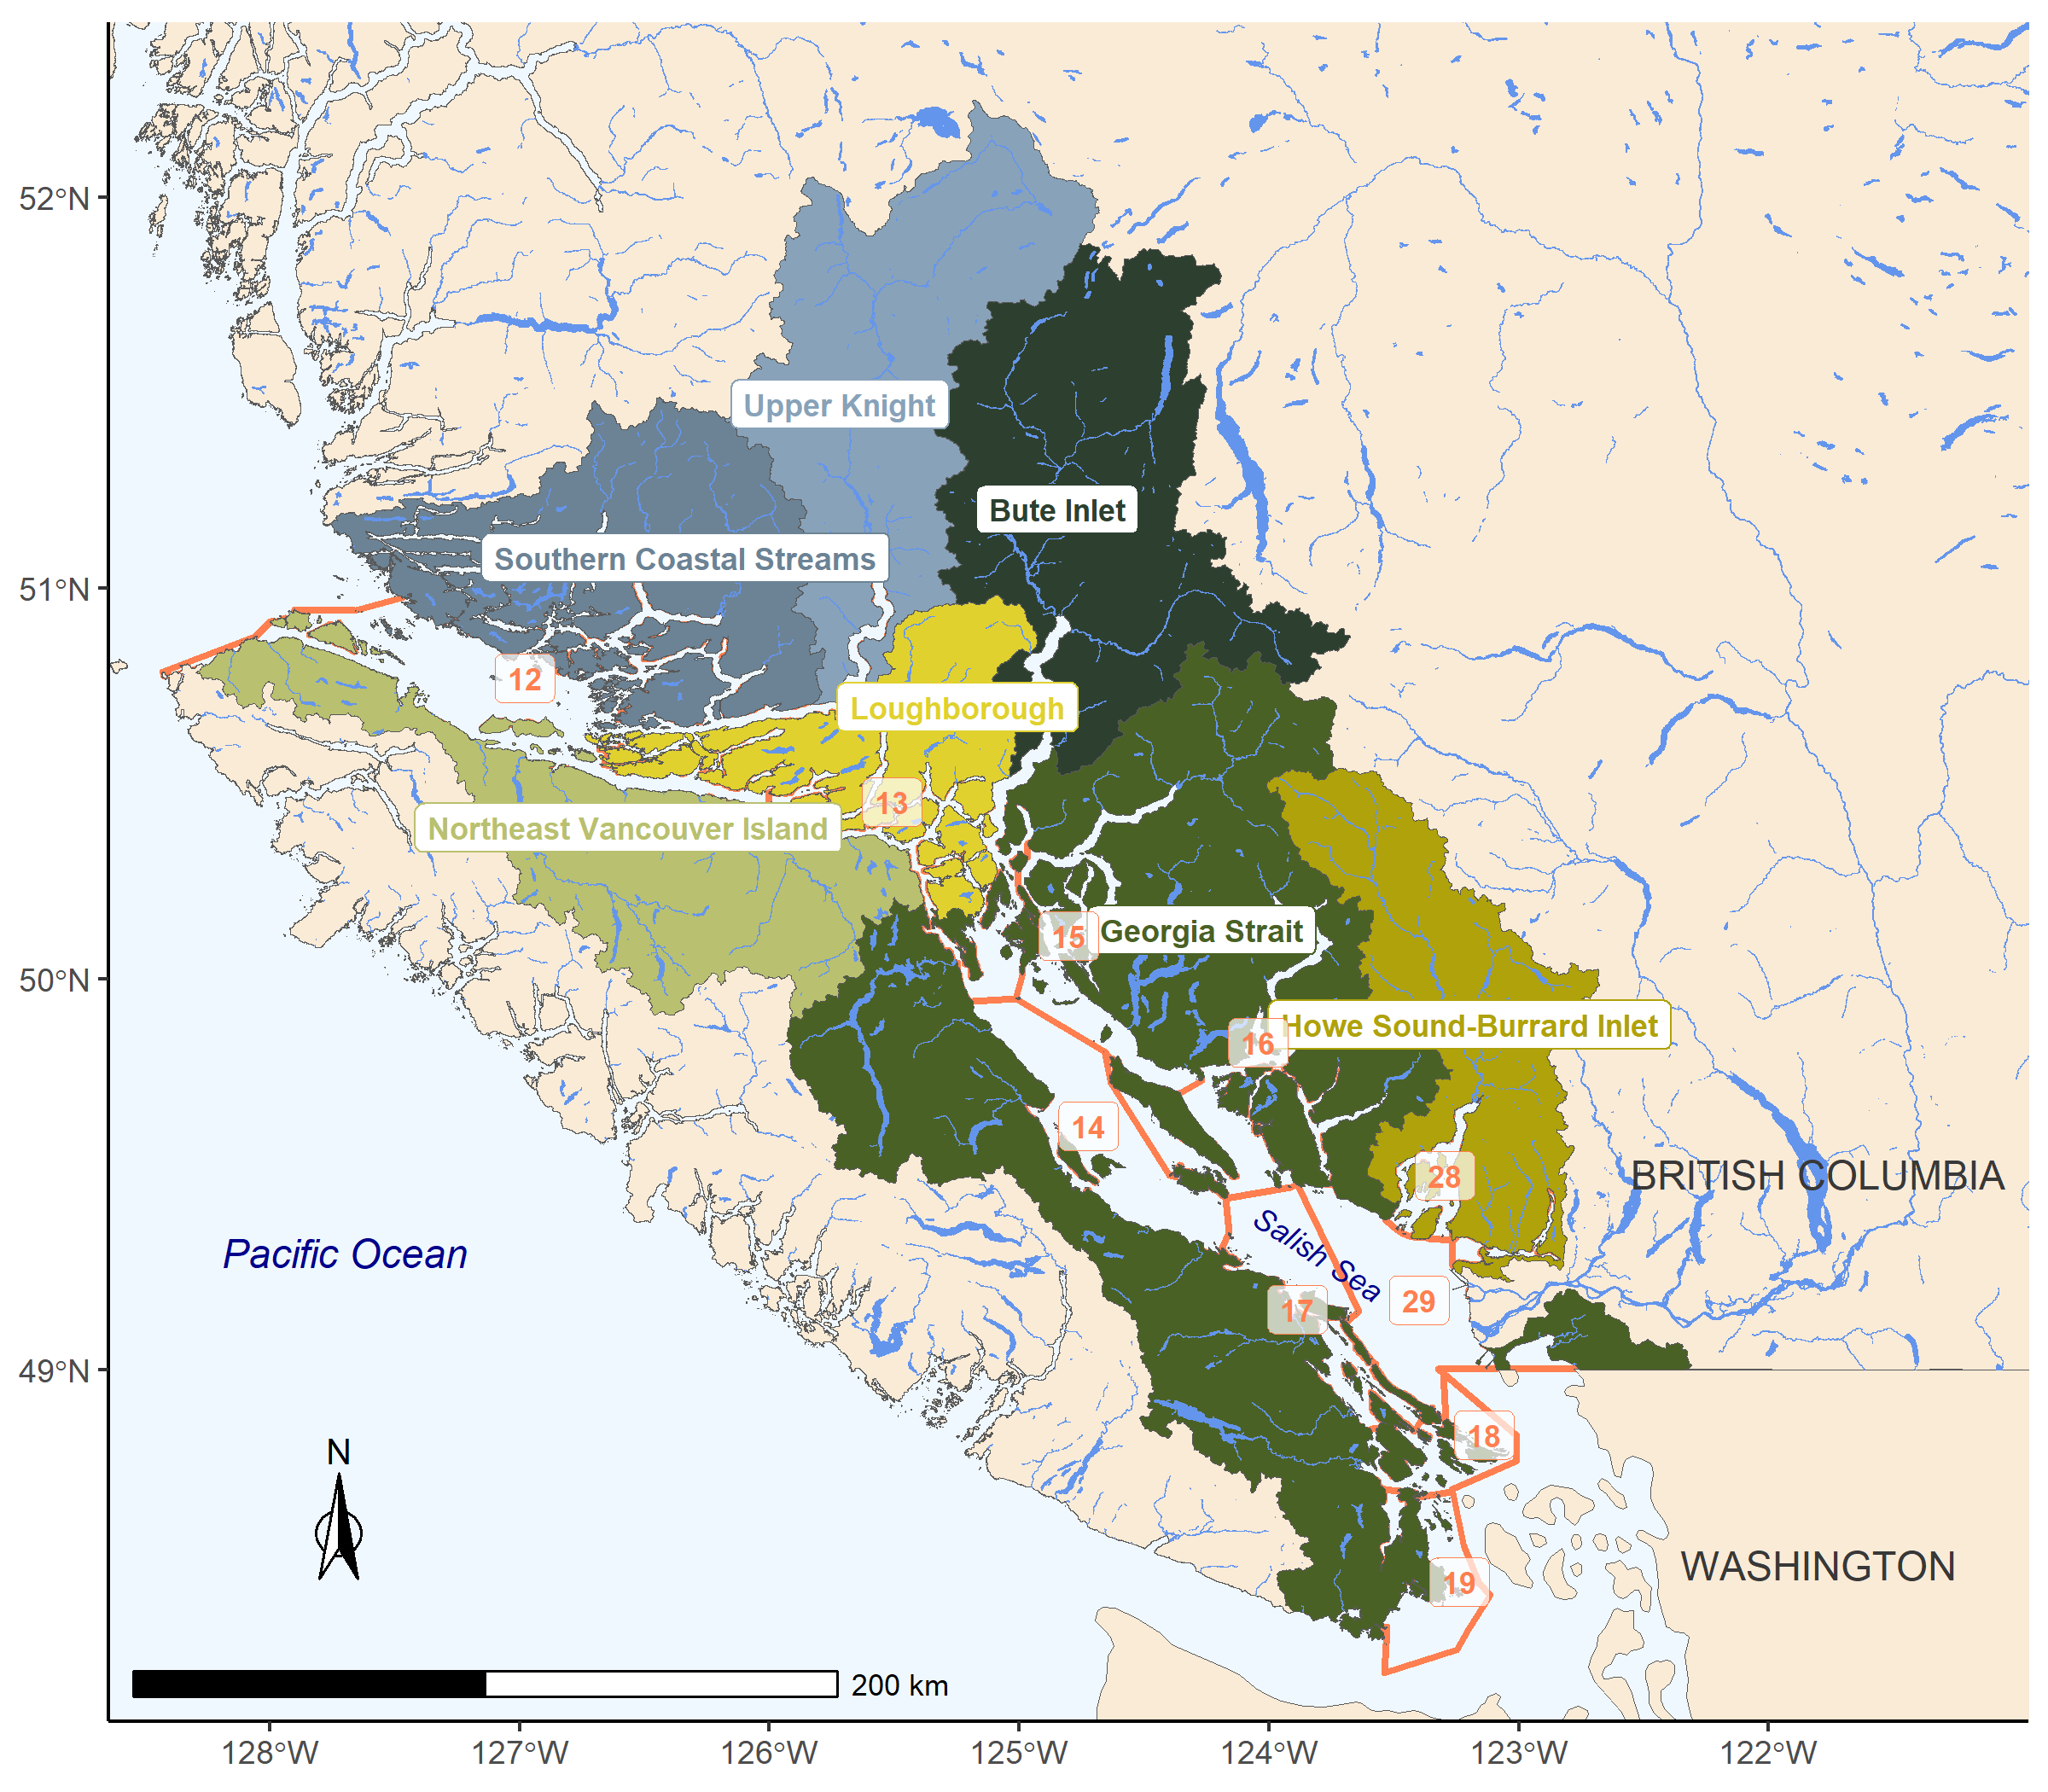
\includegraphics[width=6in]{C:/github/SalmonLRP_csasdown/caseStudyWP/figure/fig_chum_CU_map}}{Figure}

\}

\caption{The seven Conservation Units that make up the Inside South Coast Chum Stock Management unit (not including Lower Fraser and Fraser Canyon Conservation Units). Numbers indicate the Fishery Management Areas associated with these populations.}

(\#fig:chum\_map) \textbackslash end\{figure\}

\hypertarget{data-2}{%
\subsection{DATA}\label{data-2}}

We used essentially the same data used in \texttt{@holt\_evaluating\_2018}, updated with escapement data up to 2018. \texttt{@van\_will\_inner\_2014} provides more details on the data sources, infilling procedures and run reconstruction, which were reproduced for this study and described below. We did not include the Lower Fraser or Fraser Canyon chum CUs.

\hypertarget{spawner-counts-escapement}{%
\subsubsection{Spawner counts / Escapement}\label{spawner-counts-escapement}}

Most of the escapement data used comes from the NUSEDS database (a small amount from Lower Fraser Stock Assessment for Areas 28 and 29, FSC in-river catch from some First Nations and enhanced escapement from SEP) \emph{textcolor\{cyan\}\{LW: probably unneccesary detail\}}. Escapement data record the estimates of total spawners by stream and CU for each year. Biologists from Fisheries and Oceans Canada and First Nations including \ldots{} (Island Marine Aquatic Working Group) \emph{\textcolor{cyan}{LW: which ones?}} generate these data by walking streams and counting fish, and using fences or weirs on some rivers. If there was more than one count for a stream in a given year, total escapement was estimated using the area under the curve (AUC) method.

\hypertarget{fishery-harvest-genetics-and-age}{%
\subsubsection{Fishery harvest, genetics, and age}\label{fishery-harvest-genetics-and-age}}

The number of chum caught in fisheries in the Inside South Coast area were taken from the DFO Clockwork Database, which includes the DFO Fishery Operating System and Sales slip databases and Genetic Stock Identification data. Age distributions for each year were taken from the Johnstone Strait fishery aggregate, as age data for specific CUs or streams was not available.

\hypertarget{data-treatment}{%
\subsubsection{Data treatment}\label{data-treatment}}

-- Escapement data: Infilling of escapement data: (i) summarize infilling methods (ii) show plot of infilled escapement series for all 7 CUs (iii) describe that we are only using 5 CUs without CU infilling for anlayses

We removed the summer run fish as all the data in regards the reconstruction work is associated with populations that return in the fall.

To get wild escapement, we kept only wild spawners, removing hatchery spawners, spawners harvested at a facility, and spawners collected for brood stock.

We also removed spawners for the Qualicum River, Little Qualicum River, and Puntledge River, as these systems have been nearly 100\% enhanced at least since enhancement began at these locations. We have little data in the enhanced contribution found in these returns but for the purposes of removing hatchery origin fish, we make the assumption that these streams had 100\% hatchery origin spawners.

-- Recruitment data: use of run reconstruction model

The steps for preparing the data for analysis were:
\begin{enumerate}
\def\labelenumi{\arabic{enumi}.}

\item
  Infill total and wild escapement by CU and Area, (by stream for CUs with observations, by CU for years with no observations in a CU)
\item
  Add fishery catch by CU and Area to total escapement to estimate total returns / recruitment / stock \emph{\textcolor{cyan}{LW: not sure which term to use here. Recruitment might be confusing since it is recruits in a spawning year, not for a brood year}}
\item
  Use proportion of wild:total escapement by CU and Area to estimate number of wild returns
\item
  Use age proportions of catch to estimate age of returns and get recruits by brood year for each CU.
\item
  Result: wild spawners and corresponding recruits by brood year for each CU
\end{enumerate}
\hypertarget{infilling-of-spawner-escapement-data}{%
\subsubsection{Infilling of spawner escapement data}\label{infilling-of-spawner-escapement-data}}

The data we used had years where not all streams were counted. When a CU had some streams counted in a year, we infilled by stream. When there were no counts of spawners for a CU in a given year, we infilled by CU for that year and CU. We had to infill by CU to get total spawners to use for the run reconstruction, but we did not use CUs with CU-level infilling in the retrospective analysis of LRPs, as it assumes that escapement is correlated between CUs in a given year.

There were two puproses of infilling: 1. Infill total and wild escapement by CU and Area in order to get wild returns by CU and Area, in order to estimate recruits for each brood year. 2. Infill wild escapement by CU, in order to get a time series of wild escapement to use in retrospective analysis of LRPs.

\hypertarget{infilling-by-stream}{%
\paragraph{Infilling by stream}\label{infilling-by-stream}}

\hypertarget{infilling-by-cu}{%
\paragraph{Infilling by CU}\label{infilling-by-cu}}

\textbackslash begin\{figure\}{[}htb{]}

\{\centering \pdftooltip{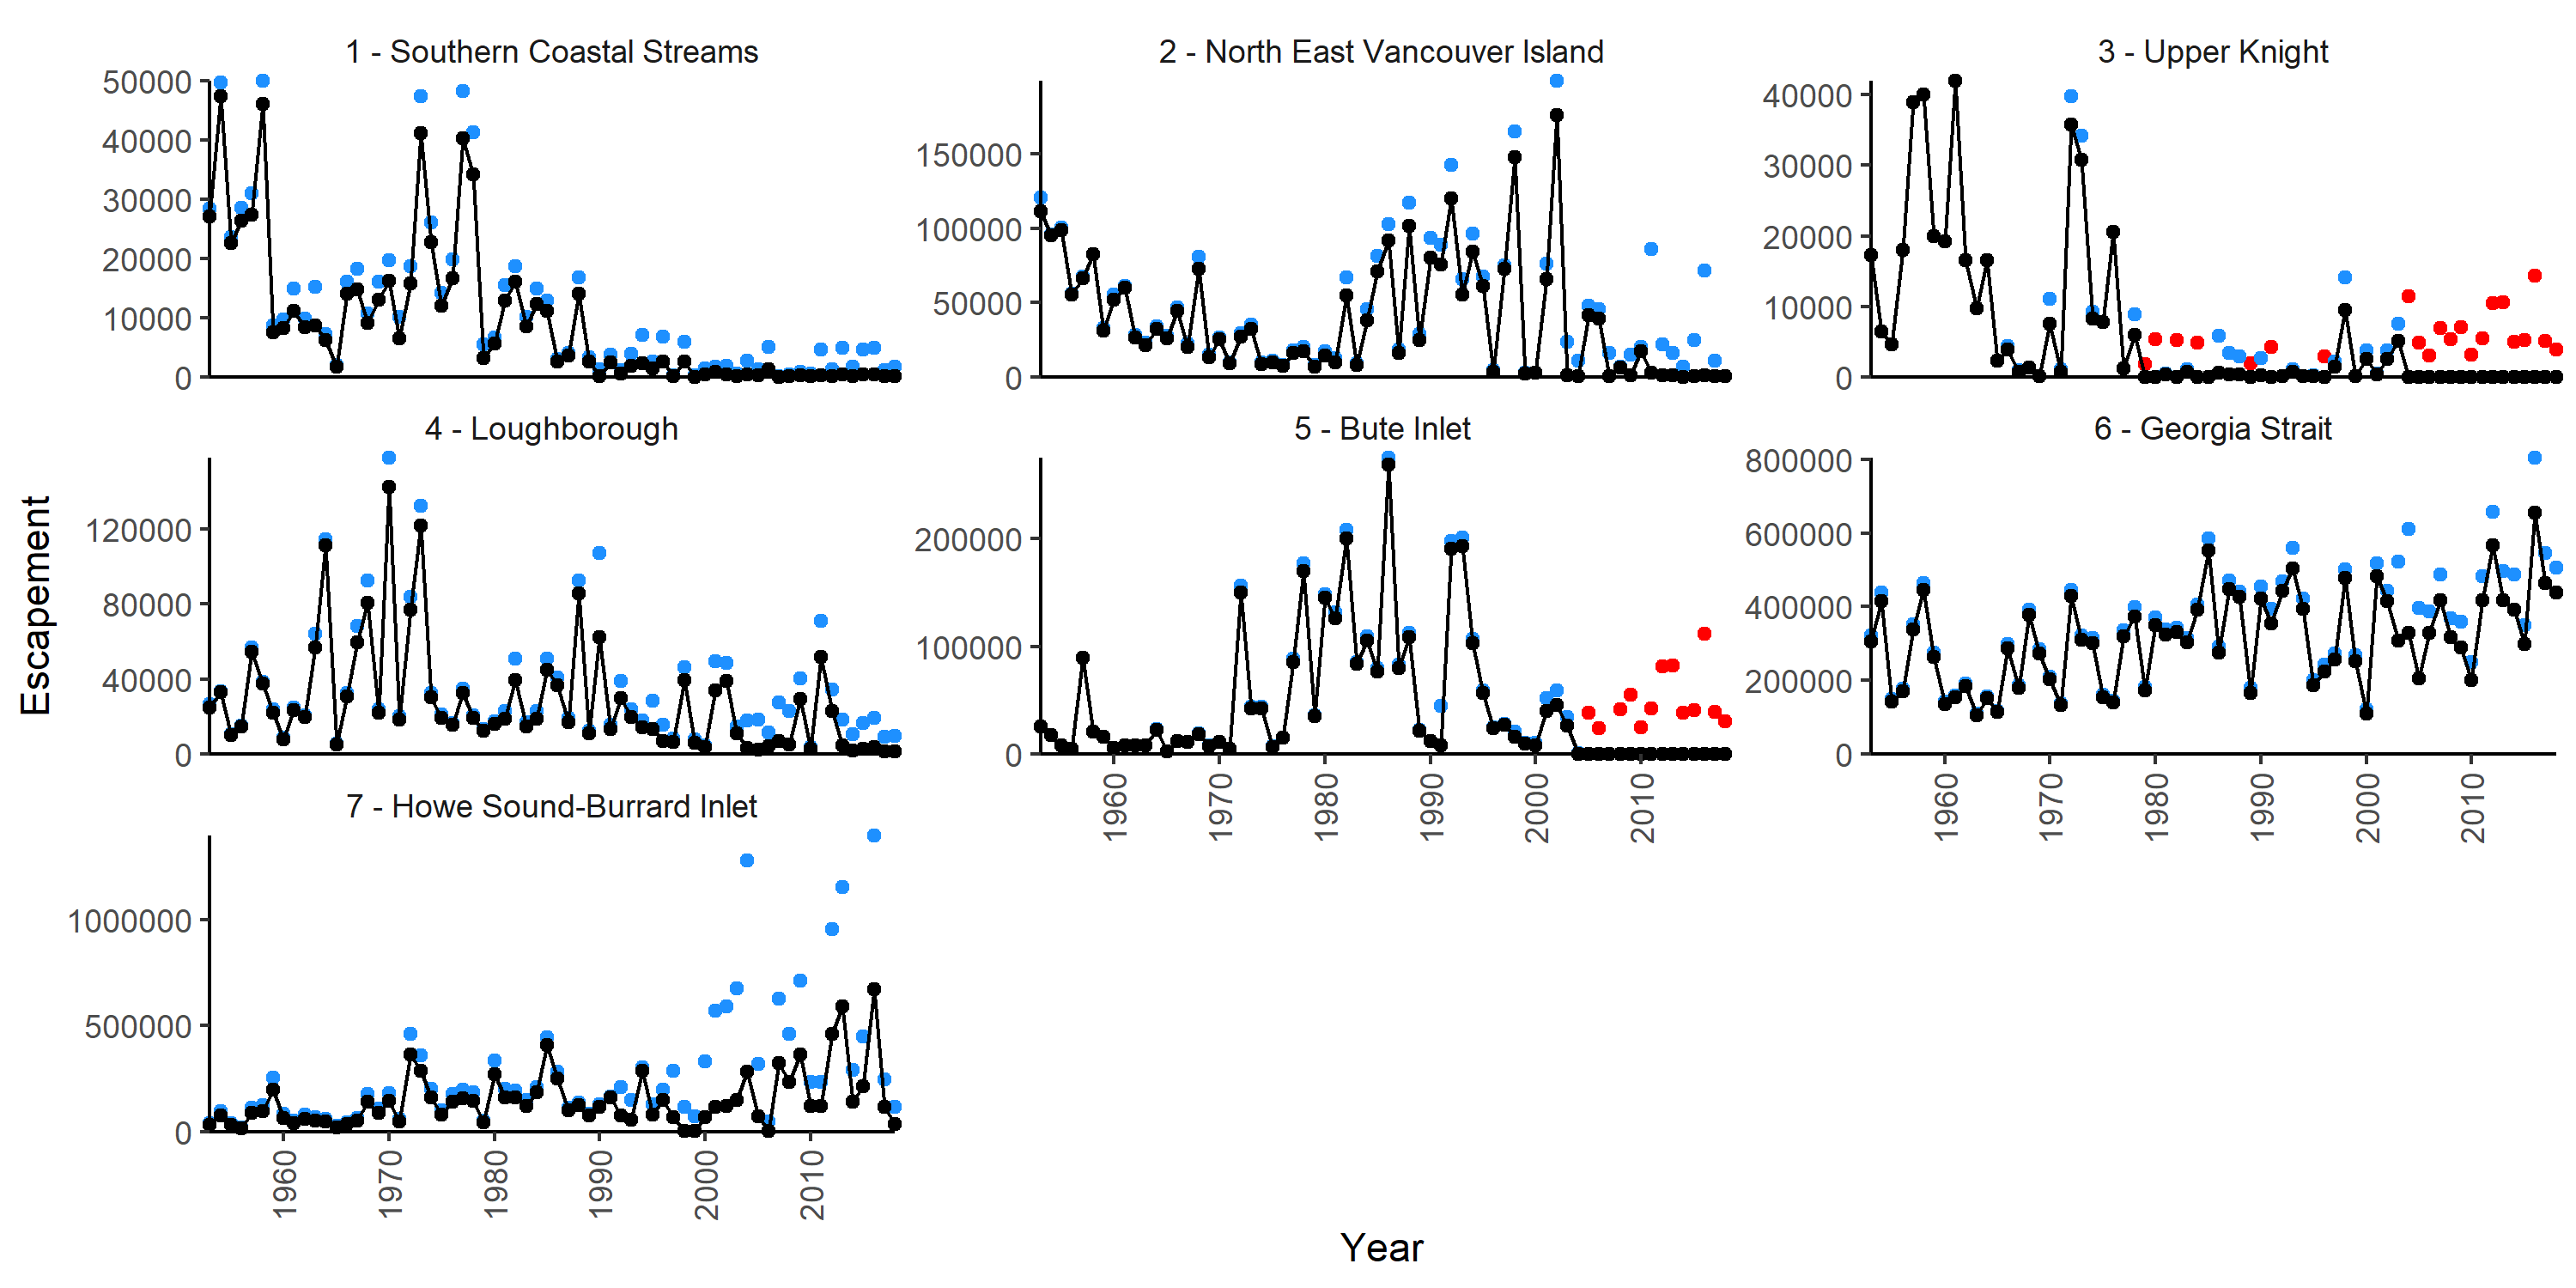
\includegraphics[width=6in]{C:/github/SalmonLRP_csasdown/caseStudyWP/figure/fig_compare_actual_infill_by_stream_and_CU}}{Figure}

\}

\caption{Chum salmon escapement for the seven Conservation Units. Black points indicate actual counts, blue points are infilled by stream, and red points are infilled by Conservation Unit.}

(\#fig:chum\_escapement\_infill) \textbackslash end\{figure\}

\hypertarget{run-reconstruction-to-estimate-recruitment}{%
\subsubsection{Run reconstruction to estimate recruitment}\label{run-reconstruction-to-estimate-recruitment}}

Data and methods are available at: \url{https://github.com/Pacific-salmon-assess/SalmonLRP_RetroEval/tree/withChum} \emph{\textcolor{cyan}{LW:Update url when withChum branch merged with main}}

\hypertarget{methods-2}{%
\subsection{METHODS}\label{methods-2}}

\hypertarget{benchmarks-for-conservation-units}{%
\subsubsection{Benchmarks for Conservation Units}\label{benchmarks-for-conservation-units}}

\hypertarget{benchmark-based-on-stock-recruit-relationship---sgen}{%
\subsubsection{Benchmark based on stock-recruit relationship - Sgen}\label{benchmark-based-on-stock-recruit-relationship---sgen}}

\hypertarget{benchmark-based-on-historical-abundance---percentile}{%
\subsubsection{Benchmark based on historical abundance - Percentile}\label{benchmark-based-on-historical-abundance---percentile}}

\hypertarget{regression-forms}{%
\subsubsection{Regression forms}\label{regression-forms}}

Bernoulli vs.~Binomial

\hypertarget{empirical-lrps-2}{%
\subsubsection{EMPIRICAL LRPS}\label{empirical-lrps-2}}
\begin{itemize}
\item
  We evaluate two empirical (data-based) approaches for developing aggregate abundance-based LRPs for Inside South Coast Chum using the 5 CUs with \textgreater{} 15 years of data {[}not sure this is the best way to descibe??; please fix{]}. Both approaches attempted to estimate LRPs by fitting logistic regression models to historically observed data; they differ in the metric used to represent CU-level lower benchmarks.
\item
  The first approach uses Sgen \ldots{}
\item
  The second approach used percentile-based benchmarks \ldots{}
\item
  Due to poor logistic model fits using the entire 19xx - 2018 time series for both Sgen and percentile benchmarks, we did not conduct retrospective analyses for this SMU. The underlying data characteristics that lead to poor logsitic model fits are highlighted in the results section below.
\end{itemize}
\hypertarget{projected-lrps-tbd}{%
\subsubsection{PROJECTED LRPS (TBD)}\label{projected-lrps-tbd}}

\hypertarget{multidimensional-approach-tbd}{%
\subsubsection{MULTIDIMENSIONAL APPROACH (TBD)}\label{multidimensional-approach-tbd}}

\hypertarget{results-2}{%
\subsection{RESULTS}\label{results-2}}

\hypertarget{empirical-lrps-3}{%
\subsubsection{EMPIRICAL LRPS}\label{empirical-lrps-3}}
\begin{itemize}

\item
  Show poor model fits for each benchmark (using Bernoulli)
\item
  Summarize model fit diagnostics
\item
  Highlight low covariance and differences in scale, and describe how these make empirical LRPs unsuitable for this SMU
\item
  Also - include plots showing variation in Sgen and percentile benchmarks over time for the 5 CUs to highlight time-varying concerns.
\end{itemize}
\hypertarget{projected-lrps-tbd-1}{%
\subsubsection{PROJECTED LRPS (TBD)}\label{projected-lrps-tbd-1}}

\hypertarget{multidimensional-approach-tbd-1}{%
\subsubsection{MULTIDIMENSIONAL APPROACH (TBD)}\label{multidimensional-approach-tbd-1}}

\hypertarget{lessons-learned-from-case-study-applications}{%
\section{LESSONS LEARNED FROM CASE STUDY APPLICATIONS}\label{lessons-learned-from-case-study-applications}}
\begin{itemize}

\item
  SYnthesize main results and conclusions from case studies
\end{itemize}
\clearpage

\hypertarget{references}{%
\section*{REFERENCES}\label{references}}
\addcontentsline{toc}{section}{REFERENCES}

\Appendices


\clearpage

\refstepcounter{chapter}
\label{app:first-appendix}
\starredchapter{APPENDIX~\thechapter. THE FIRST APPENDIX}

Content here.


\clearpage

\refstepcounter{chapter}
\label{app:second-appendix}
\starredchapter{APPENDIX~\thechapter. THE SECOND APPENDIX, FOR FUN}

More content.

\end{document}
